\subsection{\acl{ML}}
\label{subsec:MachineLearning}

\acf{ML} is a subfield in Computer Science that develops algorithms capable of automatically learn and make predictions based on data~\cite{Bishop2006}. In supervised learning, the data is retrieved from datasets or corpus, and in unsupervised learning, the data is directly sampled from the interaction. Despite not requiring handcrafted rules, these algorithms requires large amounts of quality data and good discriminative features in order to create good predicting models or classifiers. However, acquiring great amount of data may prove difficult in \ac{HRI} since it takes a great toll on the development design as it requires careful preparation, feature selection, data processing techniques, and most of all, test subjects (Figure~\ref{fig:MLDiagram}).

In addition, preliminary studies, in the intended scenario, are crucial to assess the most relevant interactions, and behavioural features we have to look before starting the training stage (see relation between the dataset and training in Figure~\ref{fig:MLDiagram}). One must take into account that excessive features may lead to redundancy (noise) contributing negatively to the quality of the classifier (overfitting). Therefore, it is recommended to use less features in order to have better generic model.

% REMOVED ADDED IF I HAVE SPACE (HALF PAGE)
%Most \ac{ML}-algorithms use eager learning techniques where the models produce global approximations to the given dataset however, there are another algorithms (e.g., $k$-nearest neighbours) that use lazy learning~\cite{Atkeson1997} to produce local approximations. These algorithms store the training dataset locally that is only used when given a test sample. Depending on the intended scenario, the latter approach may return better results. For example, eager learning may model a graph curve using a liner function (global approximation) whether lazy learning may use several liner functions (local approximations).


\begin{figure}[hbt]
  \centering
  %\begin{framed}
	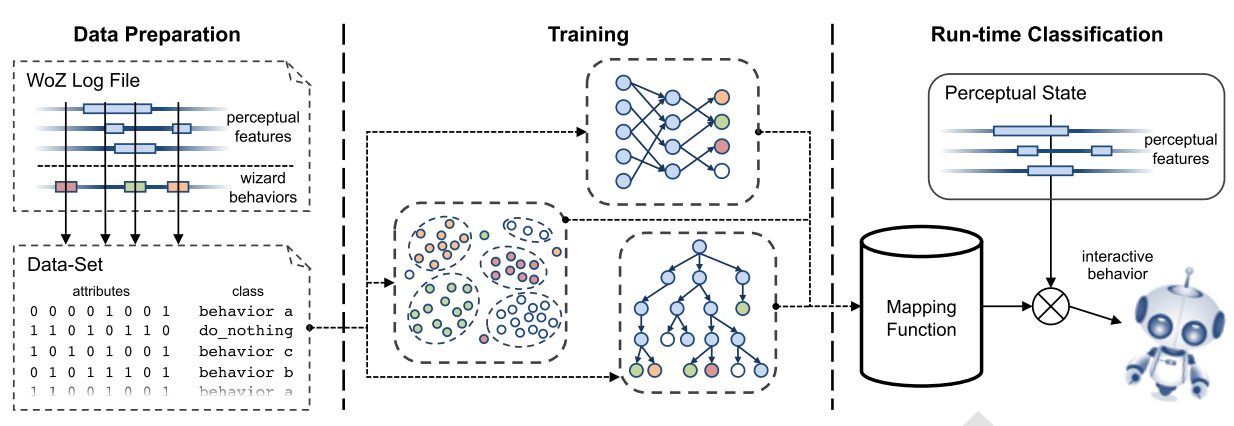
\includegraphics[width=\textwidth]{images/RestrictedPerception_ML_Diagram.png}
  %\end{framed}
  	\caption{Illustration of a \ac{ML} system in a \ac{HRI} application. The dataset is collected and prepared, then it is given to a \ac{ML} algorithm, and lastly, in run-time, the mapping function returns the most appropriate response given an input. From~\cite{Sequeira2016}.}
  	\label{fig:MLDiagram}
\end{figure}
\vspace{-3mm}

Finally, the predictive models' performance are tested using data that were not used during the training stage (test set and training set respectively). In order to limit overfitting issues, model validation techniques such as cross validation are used to test if the classifier is sufficiently generic to any given independent test dataset.

Usually, in supervised learning, the performance is measured regarding the precision (Equation~\ref{eqn:precision}) and recall (Equation~\ref{eqn:Recall}) of the generated output according to the what is expected in the corpus (TP, FP, and FN stands for True Positives, False Positives, and False Negatives, respectively).

\vspace{-9mm}
\begin{multicols}{2}
	\begin{equation}
		Precision = \frac{TP}{TP + FP}
		\label{eqn:precision}
	\end{equation}\break
	\begin{equation}
		Recall = \frac{TP}{TP + FN}
		\label{eqn:Recall}
	\end{equation}
\end{multicols}